\section{Crossing Bounds and Triangulations}
\label{sec:crossing}


Let~$G$ be undirected, and let $H$
be an even subgraph of $G$.  In this section, we describe an
algorithm to compute the minimum-cost even subgraph homologous with
$H$ in $(g+b)^{O(g+b)}n\log \log n$ time.  In fact, our algorithm can be
modified easily to compute a minimum-cost representative in
\emph{every} homology class in the same asymptotic running time;
there are exactly $2^{2g+\max\set{b-1,0}}$ such classes.
By Lemma~\ref{lem:surface-st-cut}, our algorithm can be used to find a minimum $s,t$-cut in~$G^*$ in the same amount of time.

Our algorithm closely resembles the algorithm of Chambers \etal~\cite{ccelw-scsih-08} for computing a shortest splitting cycle; in fact, our algorithm is somewhat simpler.  The first stage of our algorithm cuts the underlying combinatorial surface into a topological disk by a network of shortest paths as described in Section~\ref{sec:characterizing_crossings}.  Next, we enumerate all possible ways for an even subgraph to intersect each shortest path in the decomposition network $O(g+b)$ times.  We quickly discard any crossing pattern that does not correspond to an even subgraph in the desired homology class.  Each crossing pattern is realized by several \emph{homotopy} classes of sets of non-crossing cycles, which we easily enumerate.  Within each homotopy class, we find a minimum-length set of non-crossing cycles with each crossing pattern using an improvement by Italiano \etal~\cite{insw-iamcmf-11} to an algorithm of Kutz \cite{k-csnco-06}.  The union of those cycles is an even subgraph in the desired homology class; we return the lightest such subgraph as our output.

\note{TODO(kylejfox): Assume uniqueness of shortest paths in the prelims.}

\subsection{Crossing bound}

Our main technical lemma for this section establishes an upper bound on the number of crossings between an arbitrary shortest path and the minimum-weight even subgraph in any homology class.  Crossing-number arguments were first used by Cabello and Mohar \cite{cm-fsnsn-07} to develop the first subquadratic algorithms for shortest non-contractible and non-separating cycles in undirected surface embedded graphs; their arguments are the foundation of all later improvements of their algorithm \cite{c-mdpg-06, k-csnco-06, cce-msspe-13}.  Our proof is quite similar to the argument of Chambers \etal~\cite{ccelw-scsih-08} that the shortest \emph{splitting} cycle crosses any shortest path $O(g+b)$ times.  However, our new proof is simpler, because the structure we seek is a true subgraph, which need not be connected, rather than a single (weakly) simple closed walk.

As mentioned in Section~\ref{sec:characterizing}, we cannot consistently define when a shortest path crosses an even subgraph.  Instead, we consider the total number of crossings between a shortest path and the cycles in a cycle decomposition.

\begin{lemma}
\label{lem:crossing}
Let $G$ be an edge-weighted graph embedded on a surface with genus $g$ and $b$ boundary components.  Let $H$ be a subgraph of $G$ of minimum weight in its $\Z_2$-homology class, and let $\gamma_1, \gamma_2, \dots, \gamma_r$ be a cycle decomposition of $H$.  The total number of crossings between any shortest path in $G$ and the cycles $\gamma_1, \gamma_2, \dots, \gamma_r$ is at most $6g+2b-3$.
\end{lemma}

\begin{proof}
Let $\sigma(y,z)$ denote the shortest path between any two vertices $y$ and~$z$, and let $\sigma = \sigma(u,v)$ for some vertices $u$ and~$v$.  Uniqueness of shortest paths implies that if $y$ and $z$ are vertices of $\sigma$, either the shortest path $\sigma(y,z)$ or its reversal $\sigma(z,y)$ is a subpath of $\sigma$.  Without loss of generality, we can assume that $\sigma$ crosses each cycle $\gamma_i$ at least once.  For each $i$, let~$x_i$ denote the number of times $\sigma$ and $\gamma_i$ cross, and let $x = x_1 + x_2 + \cdots + x_r$.  We need to prove that $x\le 6g+2b-3$.

Consider the graph $G/\sigma$ obtained from $G$ by contracting $\sigma$ to a single vertex $uv$.  This graph inherits a cellular embedding on $\Sigma$ from the cellular embedding of $G$.  Each cycle $\gamma_i$ is contracted to the union of $x_i$ simple non-crossing loops in $G/\sigma$ with basepoint $uv$.  Altogether, we obtain $x$ loops, which we denote $\ell_1, \ell_2, \dots, \ell_x$.

Suppose some loop $\ell_i$ is contractible.  This loop is the contraction of a path $\pi_i$ in $G$ whose endpoints~$u_i$ and $v_i$ lie in $\sigma$.  The cycle $\delta = \pi_i \cdot \sigma(v_i,u_i)$ is also contractible.  Thus, the even subgraph $H\oplus\delta$ is homologous with $H$.  Moreover, the uniqueness of shortest paths implies that the weight of $H\oplus\delta = H \cup \sigma(v_i,u_i) \setminus \pi_i$ is smaller than the weight of~$H$.  But this contradicts our assumption that $H $ has minimum weight in its homology class.

Now suppose some pair of loops $\ell_i$ and $\ell_j$ are homotopic; by definition, the cycle $\ell_i\cdot\reverse{\ell_j}$ is contractible.  These two loops are contractions of paths $\pi_i$ and $\pi_j$ in $G$ with endpoints in $\sigma$.  Let $u_i$ and~$v_i$ denote the endpoints of $\pi_i$, and let $u_j$ and~$v_j$ denote the endpoints of $\pi_j$.  The cycle $\pi_i \cdot \sigma(v_i,v_j) \cdot \overline{\pi_j} \cdot \sigma(u_j, u_i)$ in $G$ is also contractible.  Let $\delta$ denote the set of edges of $G$ that appear in this cycle exactly once.  If the sub-paths $\sigma(v_i,v_j)$ and $\sigma(u_j, u_i)$ are edge-disjoint, then $\delta$ is a contractible cycle; otherwise, $\delta$ is the union of two non-crossing homotopic cycles.  In either case, $\delta$ is a boundary subgraph, so the symmetric difference $H\oplus\delta$ is homologous with $H$.  Moreover, $H\oplus\delta$ has smaller weight than~$H$, and we obtain another contradiction.

We conclude that the loops $\ell_1, \ell_2, \dots, \ell_x$ lie in distinct nontrivial homotopy classes.  Thus, these loops define an embedding of a single-vertex graph with $x$ edges onto $\Sigma$, where no face of the embedding is a disk bounded by less than three edges.  Euler's formula now implies that $x\le 6g+2b-3$~\cite[Lemma~2.1]{ccelw-scsih-08}.
\end{proof}

We emphasize that different cycle decompositions of the same even subgraph may lead to different numbers of crossings.  Our crossing bound applies to \emph{any} cycle decomposition.

\subsection{Triangulations and crossing sequences}

We may now describe our algorithm.
We can cut our combinatorial surface $\Sigma\setminus P$ into a $2\beta$-gon, or \emph{abstract polygonal schema}, by cutting along each path in $P$ and replacing each copy of each path in the cut surface with a single edge.  Thus, each path in $P$ corresponds to two edges of this polygon. The vertices correspond to copies of the common basepoint of $P$ if $\Sigma$ has no boundary, or to boundary paths between endpoints of $P$ otherwise.

We dualize the abstract polygonal schema by replacing each edge with a vertex, and connecting vertices which correspond to adjacent edges in the primal schema.  Any collection of non-crossing, non-self-crossing cycles corresponds to a \emph{weighted triangulation} \cite{ccelw-scsih-08}, where we draw an edge between two vertices of the dual abstract polygonal schema if and only if some cycle consecutively crosses the corresponding pair of paths in the greedy system of loops.  Each edge is weighted by the number of times such a crossing occurs in our collection.  Conversely, a weighted triangulation corresponds to a collection of non-crossing, non-self-crossing cycles as long as corresponding vertices are incident to edges of equal total weight.  Lemma~\ref{lem:crossing} implies that we only need to consider weights between 0 and $O(g+b)$.  Thus, there are $(g+b)^{O(g+b)}$ different weighted triangulations for each valid crossing vector.


\begin{figure}[htb]
\centering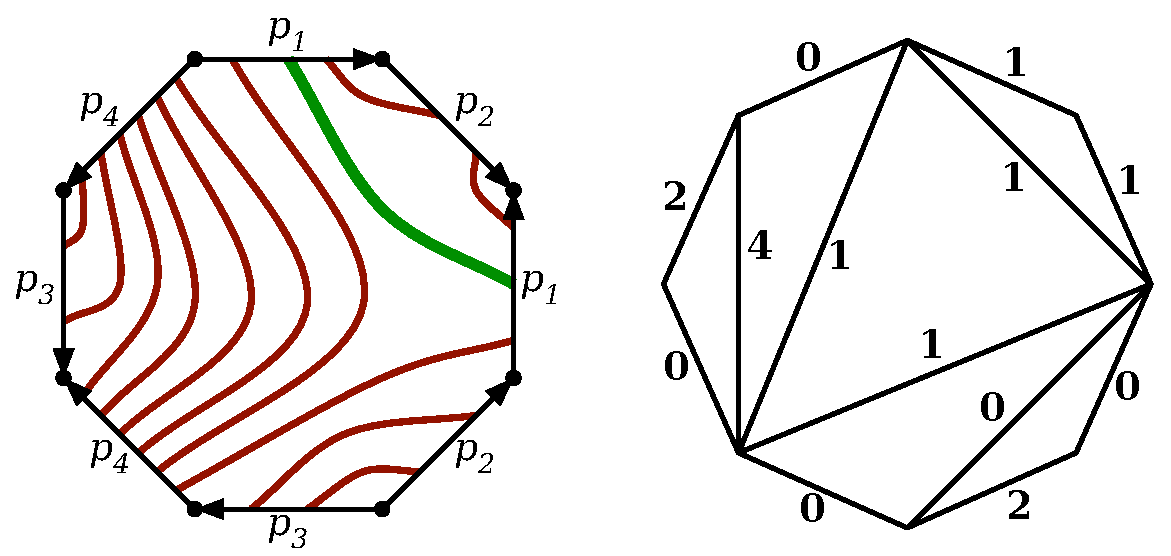
\includegraphics[height=1.45in]{Fig/triangulation}
\caption{Two disjoint simple cycles on a surface of genus 2, and the corresponding weighted triangulation.}
\end{figure}

For each valid weighted triangulation, we can compute a corresponding collection of abstract cycles in $O((g+b)^2)$ time by brute force.  In the same time, we can also compute the \emph{sequence} of crossings of each abstract cycle with the paths in $P$.  An algorithm of Kutz~\cite{k-csnco-06} computes the shortest cycle in $G$ with a given crossing sequence of length $x$ in $O(x n \log n)$ time, by gluing together $x$ copies of the planar surface $\Sigma\setminus P$ into an annulus and calling Frederickson's planar minimum-cut algorithm \cite{f-faspp-87}.
Italiano \etal~\cite{insw-iamcmf-11} point out that their recent $O(n \log \log n)$-time improvement in computing minimum $s,t$-cuts in planar graphs can be used instead of Frederickson's algorithm. 
Thus, for each weighted triangulation, we obtain the shortest corresponding set of cycles in $O((g+b)^2 n \log \log n)$ time.

\begin{theorem}
Let $G$ be a graph with positively weighted edges embedded on a surface with genus
$g$ and $b$ boundary components, and let $H$ be an even subgraph of $G$.
We can compute the minimum-cost even subgraph homologous with $H$ in
$(g+b)^{O(g+b)} n\log \log n$ time.
\end{theorem}

\begin{corollary}
Let $G$ be an edge-weighted graph embedded on a surface with genus $g$ and $b$ boundary components, and let $s$ and $t$ be vertices of $G$.  We can compute the minimum-weight $(s,t)$-cut in $G$ in $g^{O(g)} n\log \log n$ time.
\end{corollary}
